%%%%%%%%%%%%%%%%%%%% author.tex %%%%%%%%%%%%%%%%%%%%%%%%%%%%%%%%%%%
%
% sample root file for your "contribution" to a proceedings volume
%
% Use this file as a template for your own input.
%
%%%%%%%%%%%%%%%% Springer %%%%%%%%%%%%%%%%%%%%%%%%%%%%%%%%%%


\documentclass{svproc}
%
% RECOMMENDED %%%%%%%%%%%%%%%%%%%%%%%%%%%%%%%%%%%%%%%%%%%%%%%%%%%
%

% to typeset URLs, URIs, and DOIs
\usepackage{url}
\def\UrlFont{\rmfamily}

%%%%%%%%%%%%%%%%%%%%%%%%%%%%%%%%%%%%%%%%%%%%%%%%%%%%%%%%%%%%%%%%%%%%%%%%%%%%%%%%%%%%%%%%%%
%
%%%%%%%%%%%%%%%%%%%%%%%%%%%%%%%%%%%%%%
% jmejia added
\usepackage{amsmath,amssymb}
\usepackage{graphicx}
\usepackage{algorithm, algpseudocode}
% \graphicspath{{img/}}
%%%%%%%%%%%%%%%%%%%%%%%%%%%%%%%%%%%%%%
\begin{document}
\mainmatter              % start of a contribution

\title{A New Evolutionary Optimization Method Based on Center of Mass}
%
\titlerunning{Evolutionary Centers Algorithm}  % abbreviated title (for running head)

\author{J. A. Mej\'ia de-Dios\inst{1} \and Efr\'en Mezura-Montes\inst{1}}
%
\authorrunning{Mej\'ia de-Dios and Mezura-Montes} % abbreviated author list (for running head)
%
\institute{%
Artificial Intelligence Research Center, \\
University of Veracruz, \\
Sebasti\'an Camacho 5, Centro \\
Xalapa, Veracruz, 91000, M\'exico, \\
WWW home page: \texttt{https://www.uv.mx/ciia/}
}

\maketitle

\begin{abstract}
Physical phenomena have been the inspiration for proposing different
optimization methods such as electro-search algorithm (ES), central force 
optimization (CFO), and charged system search (CSS) among others. This work presents a new 
optimization algorithm based on some principles from physics and
mechanics, which is called Evolutionary Centers Algorithm (ECA). We utilize 
the center of mass definition for creating new directions for moving the worst 
elements in the population,  based on their objective function values, %
to better regions of the search space.  The efficiency of the new approach is showed by using the 
CEC 2017 competition benchmark functions. We present a comparison against the best algorithm (jSO) 
in such competition.  The results obtained are promising.
\keywords{Optimization, center of mass, evolutionary algorithm, physics-inspired}
\end{abstract}

\section{Introduction}
Nowadays, real-world optimization problems  are complex to solve due to 
different sources of difficulty, e.g., highly  non-linear objective function 
and constraints and large number of variables. There are several population-based 
algorithms, which are competitive to solve optimization problems \cite{easSurv}.  
Two main  types can be distinguished:  evolutionary algorithms (EAs), e.g., genetic algorithms, 
differential evolution, etc., \cite{jso2017,melanie96,ed1995} and swarm 
intelligence, e.g., artificial bee colony, ant system, particle swarm optimization, etc.
\cite{abc2005,pso1995}. In this work, we are focused on EAs.\\

EAs have provided successful results when solving complex bound-constrained 
optimization problems \cite{ed1995}.  However, most popular EAs usually are 
those which design keeps simple and their number of parameters is low so 
as to facilitate the fine-tuning process when a particular problem is solved. 
\\

Motivated by the above mentioned, we propose a  physics-inspired algorithm 
based on the center of mass concept on a $D$-dimensional space for  
real-parameter single-objective optimization. The general idea is to promote 
the creation of an irregular body using $K$ mass points in the current population, 
then the center of mass is calculated to get a new direction for the next population.\\

Single-objective optimization problems are defined as follows: for a 
objective function $f(\vec{x})$, an algorithm needs to find the variables of a vector $\vec{x}$ 
that minimizes or maximizes the function $f$. It is assumed that the number 
of variables in $\vec{x}$ is $D$, i.e., $\vec{x} = (x_1,\; x_2 , \ldots , x_D )$. 
The search space is assumed to be convex, where each variable has its  boundaries 
$x_{j, \min}, \;  x_{j, \max} $ for $j = 1,\; 2,\; \ldots,\; D$. Problems are often 
found where the objective function is not explicitly known, then classical optimization 
methods in this type of problem are hardly applicable \cite{problemas}.\\

There are different algorithms based on biological or physical metaphors with 
different characteristics. Some of them use the current population distribution 
to generate new solutions, i.e., swarm intelligence algorithms such as particle 
swarm optimization (PSO) \cite{pso1995}, and the artificial bee colony (ABC) \cite{abc2005}. 
There are also algorithms inspired by physical phenomena such as Newton's Law of 
Universal Gravitation (CFO) \cite{fisicaSurvey,cfo2007}. The relationship among those  
algorithms  is their mathematical formulation for generating solutions 
through an iterative process:
%
\begin{equation}
	\vec{x}_{i + 1} = \vec{x}_{i} + \vec{v}_{i + 1}
	\label{eqn:xxv}
\end{equation}
%
where each algorithm updates $\vec{v}_{i+1} $ as follows:
\begin{itemize}
	\item PSO:
		$$
			\vec{v}_{i + 1} = \omega \vec{v}_{i} +  
					c_1 r_{1, i} ( \vec{x}_{pbest, i} - \vec{x}_i ) + 
					c_2 r_{2, i} ( \vec{x}_{gbest, i} - \vec{x}_i ),
		$$
		where $\omega$ is a inertia weight used for balancing the global search 
		and local search, $c_1$ and $c_2$ are two positive constants, $r_{1, i},\; r_{2, i}$ 
		are random numbers with uniform distribution in the range [0, 1].
	%%%%%%%%%%%%%%%%%%%%%%%%%%%%%%%%%%%%
	\item ABC:
		$$
			\vec{v}_{i + 1} = \phi_i (\vec{x}_i - \vec{x}_{r}),
		$$
	where $\phi_i$ is a randomly produced number with uniform distribution 
	in the interval $[-1,\;1]$.
	%%%%%%%%%%%%%%%%%%%%%%%%%%%%%%%%%%%%
	\item CFO: $$
		\vec{v}_{i + 1} = \omega \vec{v}_{i} + {\lambda \vec{F}_{i}} / {m_i},
		$$
		where $\lambda$ is a uniformly distributed random variable in [0, 1], $\omega$ 
		is user-defined weight $0 < \omega < 1$, $m_i,\; F_i$ are mass and force 
		functions, respectively, both defined by the authors.
\end{itemize}
%
%
In the three previous cases, the $\vec{v}$ value  depends of the population 
distribution at current generation $i$.\\

The following Section \ref{sec:eca} describes our algorithm and how it 
relates to what has been  described above. Section \ref{sec:results} 
presents the results obtained.  Section \ref{sec:conclusions} summarizes 
our conclusions and Section \ref{sec:further_work}  indicates the future work. 

\section{ECA} % (fold)
\label{sec:eca}
%
%
We present ECA details. First, we introduce the center of mass in physics 
terms \cite{kleppner73,serway}.

\begin{definition}
	The center of mass is the unique point $\vec{c}$ at the center of a distribution
	of mass $U = \{\vec{u}_1,\; \vec{u}_2 , \ldots , \vec{u}_K \}$ in a space that 
	has the property that the weighted sum of position vectors relative to this point 
	is zero. That is:

	\begin{equation}
		\sum_{i = 1}^K m(\vec{u}_i) (\vec{u}_i - \vec{c}) = 0, \;\; \text{ implies } \;\; 
		%%%%%%%%%%%%%%%%%%%%%
		\vec{c} = \dfrac{1}{M} \sum_{i = 1}^K  m(\vec{u}_i)  \vec{u}_i,
		\label{eq:masscenter}
	\end{equation}
	%
	%
	where $m(\vec{u}_i)$ is the mass of $\vec{u}_i$ and  $M$ is the sum of the 
	masses of vectors in $U$. Here, $m$ is a non-negative function.
\end{definition}
%
%
\begin{note}
Similar as in Statistics, the center of mass is the mean location of a distribution 
of mass in space.
\end{note}
% 
The concept of \textit{center of mass} is, by far, not new. It was introduced by the ancient 
Greek physicist, mathematician, and engineer Archimedes of Syracuse. Archimedes 
worked with some assumptions about gravity in a uniform field, so as to 
get the mathematical properties of what we now call the center of mass \cite{kleppner73}.\\

For this work, the following proposition is required for ensuring stability and keep ECA 
solutions into the convex space.

\begin{proposition}
	If $\vec{c}$ is the center of mass of a system of particles $U$, 
	then  for all $ \vec{u}\in U $:
	$$  d(\vec{c},\; \vec{u} )  \leq \text{diam}(U). $$
	%
	Here, diam$(U) := \sup\{ d(\vec{u},\; \vec{v} ) \; | \; \vec{u} ,\; \vec{v} \in U \}$.
\end{proposition}
%
\noindent
In others words, the center of mass of $U$ is never out of the minimum convex set that 
contains $U$. We are assuming Euclidean distance and $U \subset \mathbb{R}^D$ \cite{rudin}.\\

%
% 
%

In this work, the objective function of the optimization problem represents 
the mass of each solution in the population,  i.e., we set $f = m$. 
Without loss of generality, we assume that we want to maximize 
the non-negative function $f$.




\subsection{Algorithm Description} % (fold)
\label{sub:algorithm_description}

For each solution $\vec{x}_i $ in the population $P = \{ \vec{x}_1, \vec{x}_2, \ldots, \vec{x}_{N} \} $ of $N$ 
solutions, we select a subset $U \subset P $ with $K$ solutions; then, 
from $U$ we obtain the center of mass $\vec{c}$. After that, based on 
a randomly chosen solution $\vec{u}_r \in U$,  
and the already generated center of mass $\vec{c}$, we generate a direction 
to locate a new solution $ \vec{h}_i$. We suggest using the following strategy:

\begin{equation}
	\vec{h}_i = \vec{x}_i + \eta _{i} ( \vec{c}_i - \vec{u}_{r} ),
	\label{eqn:vcu}
\end{equation}
%
where 
%
\begin{equation}
	\vec{c}_i = \dfrac{1} {W} \sum_{u \in U} f(\vec{u}) \cdot \vec{u} , 
			\hspace{0.5cm} 
			W = \sum_{ \vec{u} \in U} f(\vec{u}).
	\label{eqn:center}
\end{equation}

\begin{note}
	If $f$ is constant, then the center of mass of $U$ is the geometric 
	center of  $U$. That is, assume that $f(\vec{x}) = \alpha$ for every 
	$\vec{x} \in \mathbb{R}^D$,  with $\alpha$ a positive constant. The 
	center of mass is:
%
\begin{equation}
	\vec{c}_i = \dfrac{1} {K \alpha} \sum_{ \vec{u} \in U} \alpha \cdot \vec{u} =  \dfrac{1} {K } \sum_{\vec{u} \in U} \vec{u}.
	\label{eqn:center-geometric}
\end{equation}
%
Thus, for a constant mass function, we have the center of mass converging 
to the geometric center. In real world problems, functions can be flat 
in some regions, then this algorithm may find some difficulties  when 
dealing with such issue.
\end{note}

\begin{figure}%[!ht]
	\centering
	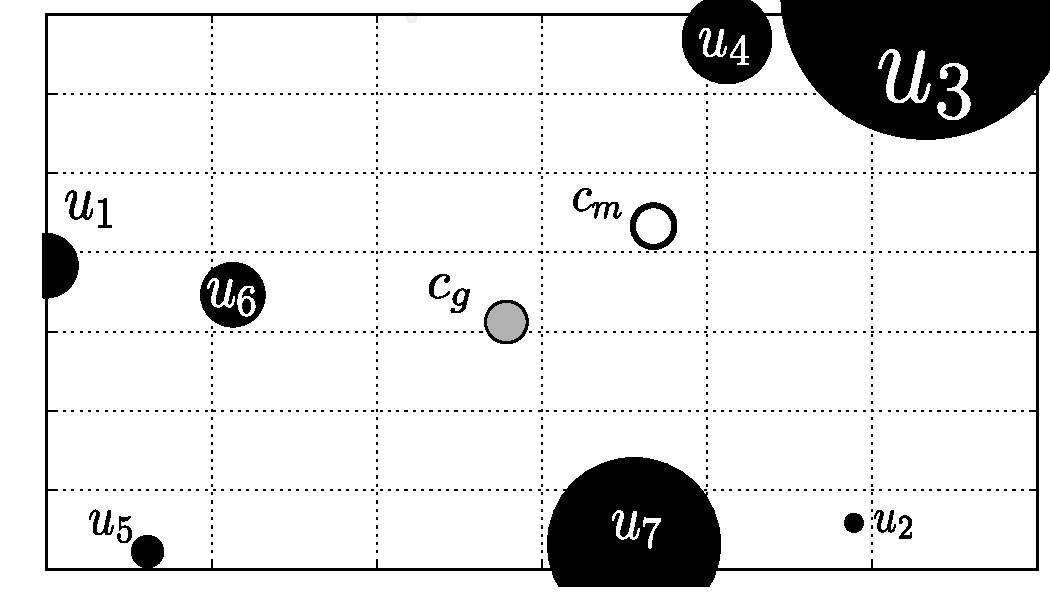
\includegraphics[width=7cm]{img/masses.pdf}
	\caption{$c_m$ is center of mass, $c_g$ is geometric center of black points. %
	Black point radius is its mass. Note the bias given by the weighted sum.}
	\label{fig:masses}       % Give a unique label
\end{figure}

\begin{note}
The bias is given by Equation (\ref{eqn:center}) because for a solution 
with the highest mass, the position of the center of mass is nearest to 
its position, see Figure \ref{fig:masses}.
\end{note}

\begin{figure}%[!ht]
	\centering
	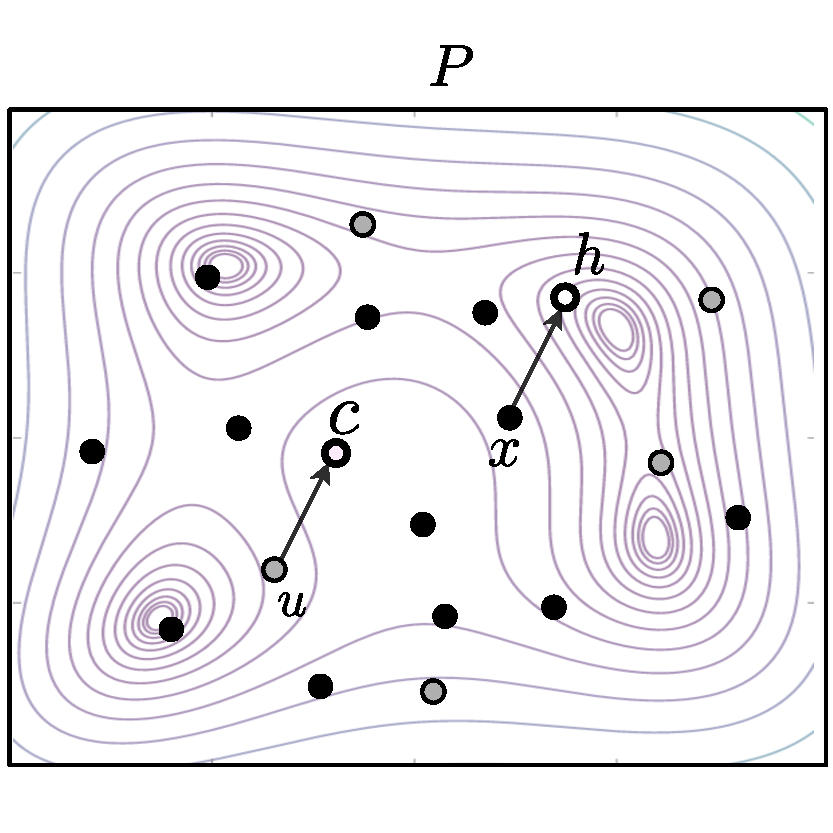
\includegraphics[width=7cm]{img/ecaG.pdf}
	\caption{Schematic diagram representing a generation of ECA. Gray points % 
	represent elements in $U$.}
	\label{fig:ecag}       % Give a unique label
\end{figure}

\begin{algorithm}%[!ht]
	\caption{ECA pseudocode}
	\label{algoritmoEca}
	\begin{algorithmic}[1]
		\Procedure{ECA}{$K = 7, \; \eta_{\max} = 2$}
		%\State poplulation size = 20 $\times$ dimension
		\State $N \gets 2K * D$
		\State Generate and evaluate start population $P$ with $N$ elements
		\While{the end criterion is not achieved}
			\State $A = \emptyset$
			\For {each $\vec{x}$ in $P$}
				\State Generate $U \subset P$ such that  card$(U) = K$
				\State Calculate $\vec{c}$ using $U$ with (\ref{eqn:center})
				\State $\eta \gets \text{rand}(0,\; \eta_{\max}) $ 
				\State $\vec{h} \gets \vec{x} + \eta  * (\vec{c} - \vec{u}) $ where $ \vec{u} \in U $ random
				
				\If{$ f(\vec{x}) < f(\vec{h})  $}
					\State Append $\vec{h} $ in $A$
				\EndIf
			\EndFor
			\State $P \gets $ best elements in $P \cup A$
			% \State 
		\EndWhile
		\State Report best solution in $P$
		\EndProcedure
	\end{algorithmic}
\end{algorithm}

Note that ECA  has only two parameters: the number of neighbors $K$ and 
the stepsize $\eta_{\max}$.  For large $K$ values, ECA could converge 
faster, we suggest $K = 7$, a value obtained experimentally. Figure \ref{fig:ecag} 
shows a representation of ECA solution update. 

\subsection{Experiments} % (fold)
\label{sub:experiments}

Algorithm \ref{algoritmoEca} details the procedure for the implementation 
of ECA. Such algorithm was coded in C language using a PC  with 
quad-core 2.4 GHz CPU and 8 GB of RAM and it was tested in thirty 
functions of CEC 2017 competition on real-parameter single-objective optimization \cite{cec2017}.\\


\begin{table}%[!ht]
	% \centering
	\caption{Representative functions from CEC 2017 benchmark. This set of %
	functions are shifted  and rotated. The search range is $[-100,\; 100]^D$.}
	\label{tab:funcs}
	\begin{tabular}{llcc}
		\hline
		Function & Formula  & Optimal  \\ \hline
		Bent Cigar Function & $ \displaystyle f_1(\vec{x}) = x_1 + 10^6 \sum_{i=2}^D x_i^2 $  & 100 \\ \hline
		%%%%%%%%%%%%%%%%%%%%%%%%%%%%%%%%%%
		Sum of Different Power Function & $ \displaystyle f_2(\vec{x}) = \sum_{i=1}^D |x_i|^{i+1} $  & 200 \\ \hline
		%%%%%%%%%%%%%%%%%%%%%%%%%%%%%%%%%%
		Zakharov Function & $ \displaystyle f_3(\vec{x}) =  \sum_{i=1}^D x_i^2 + \left(\sum_{i=1}^D 0.5x_i\right)^2 + \left(\sum_{i=1}^D 0.5x_i\right)^4 $  & 300 \\ \hline
		%%%%%%%%%%%%%%%%%%%%%%%%%%%%%%%%%%
		Rastrigin Function & $ \displaystyle f_5(\vec{x}) =  10D + \sum_{i=1}^D (x_i^2 - 10\cos(2\pi x_i)) $  & 500 \\ \hline
		%%%%%%%%%%%%%%%%%%%%%%%%%%%%%%%%%%
		High Conditioned Elliptic Function & $ \displaystyle f_{11}(\vec{x}) =  \sum_{i=1}^D (10^6)^{\dfrac{i-1}{D-1}} x_i^2 $  & 1100 \\ \hline
		%%%%%%%%%%%%%%%%%%%%%%%%%%%%%%%%%%
		Discus Function & $ \displaystyle f_{12}(\vec{x}) = 10^6 x_1^2 +\sum_{i=2}^D x_i^2 $  & 1200 \\ \hline
		%%%%%%%%%%%%%%%%%%%%%%%%%%%%%%%%%%
		Griewank’s Function & $ \displaystyle f_{15}(\vec{x}) =  \sum_{i=1}^D \dfrac{x_i^2}{4000} - \prod_{i=1}^D \cos\left( \dfrac{x_i}{\sqrt{i}} \right) + 1 $  & 1500 \\ \hline
		%%%%%%%%%%%%%%%%%%%%%%%%%%%%%%%%%%
	\end{tabular}
\end{table}


For this experimentation, $D = 10$ was considered. Here, the optimal values for the test 
functions are known (see Table \ref{tab:funcs} where representative functions are shown). There is also a maximum number of 
evaluations equal to \textit{max\_nfes} $= D \times 10,000$.\\

The parameters in all experiments were: $K = 7$, $\eta_i$ is a uniform random number 
between in (0, 2]. The size of the population was $N = 2K * D $.

% subsection algorithm_description (end)


% subsection experiments (end)

% section eca (end)



\section{Results} % (fold)
\label{sec:results}

The statistical results obtained by ECA are reported in Table \ref{tab:eca}. 
It is worth noting  that ECA obtained results close the optimum values 
while reporting low standard deviation values. Therefore, ECA behavior can 
be considered as robust and suitable to deal with different type of search spaces. 
Furthermore, we compared ECA against the most competitive algorithm in 
the CEC 2017 competition on real-parameter single-objective optimization (jSO), 
which is an adaptive algorithm based on differential evolution. The comparison 
based on 51 independent runs by each algorithm is presented in Table \ref{tab:jso}. 
As we can see, ECA, based on the 95\%-confidence Wilcoxon Rank-Sum test, 
was able to outperform jSO in five test functions, it reached similar 
results in seven test problems, and finally ECA was outperformed by jSO 
in eighteen functions. ECA was then competitive in twelve test problems. 
Moreover, ECA is more simple to implement than jSO and requires less 
mechanisms to operate.\\

Figure \ref{fig:converg} shows ECA convergence graphs. Those plots show that 
ECA is able to converge fast in most cases, which can be suitable for 
computationally-expensive real-world optimization problems.  

\begin{figure}%[!ht]
\centering
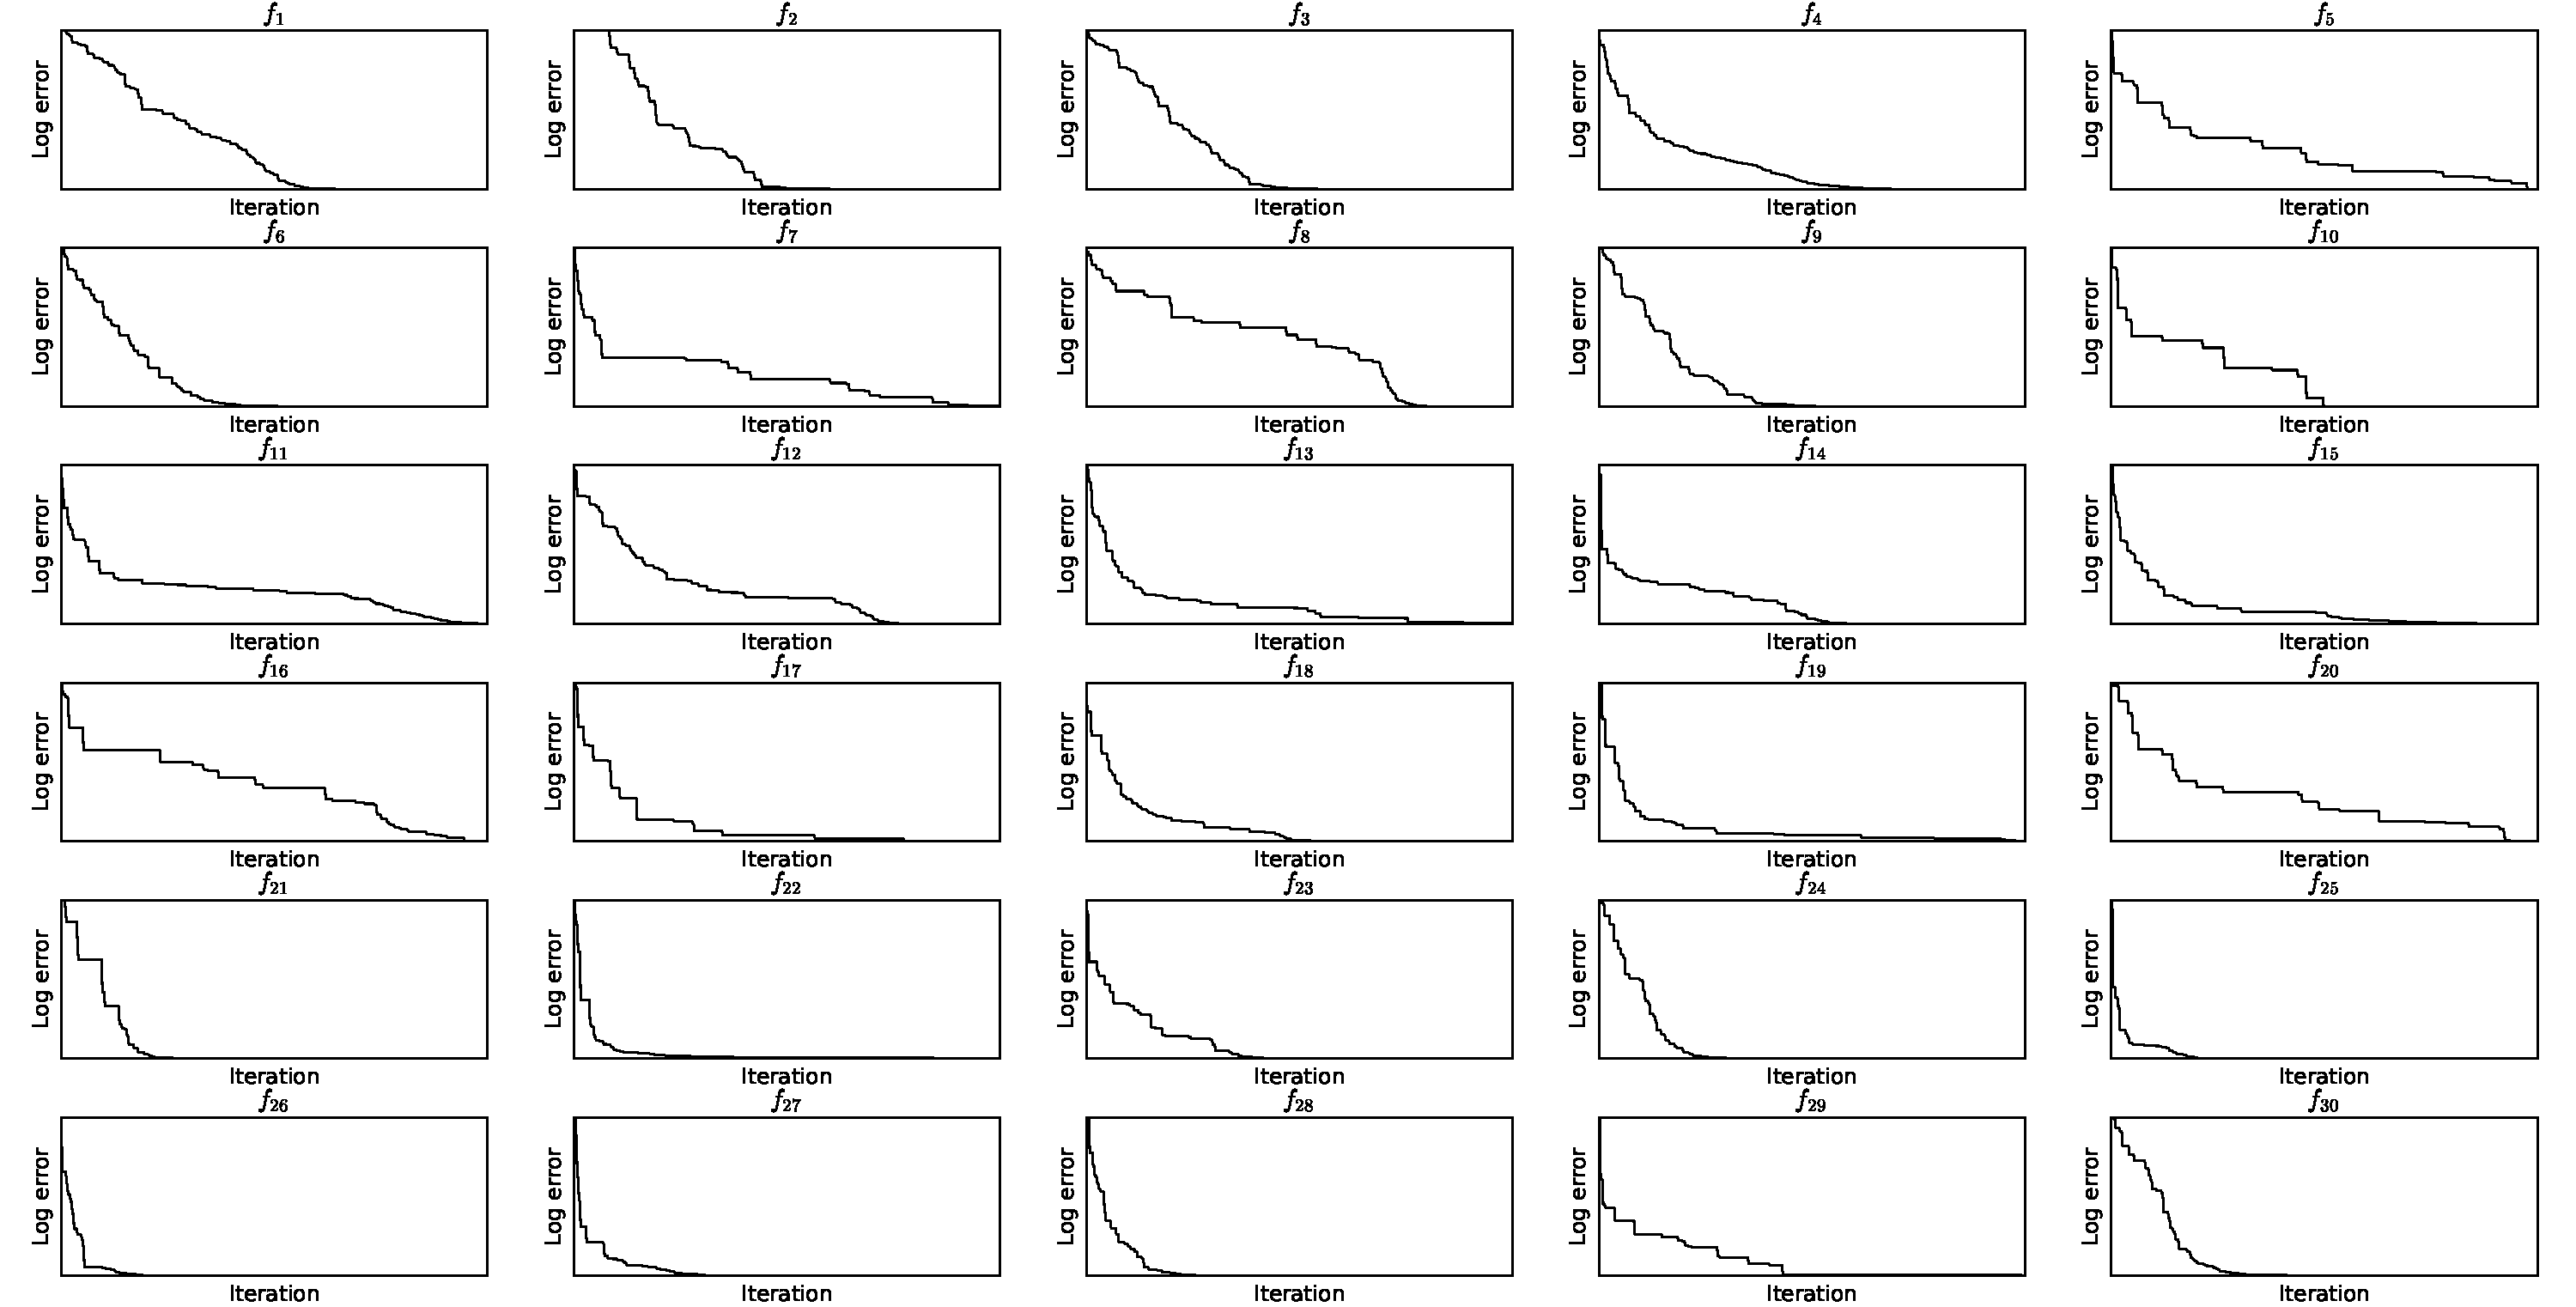
\includegraphics[width=\linewidth]{img/converg.pdf}
\caption{Convergence graphs at the run located in the median of 51 independent  runs. Log scale is used for visualization purposes.}
\label{fig:converg}       % Give a unique label
\end{figure}
%
%
\begin{table}%[!ht]
\centering
\caption{Results of 51 independent runs of ECA on CEC17 problems for $D=10$.}
\label{tab:eca}
\scalebox{0.7}{
	\renewcommand{\arraystretch}{1.3}
	\begin{tabular}{p{1cm}p{2.5cm}p{2.5cm}p{2.5cm}p{2.5cm}p{2.5cm}}
		\hline
		% \noalign{\smallskip}
		$f$ & Best & Worst & Median & Mean &  Std. \\
		\hline
		% \noalign{\smallskip}\svhline\noalign{\smallskip}
		$f_{1}$ & 0.00000E$+$00 & 0.00000E$+$00 & 0.00000E$+$00 & 0.00000E$+$00 & 0.00000E$+$00 \\ \hline
		$f_{2}$ & 0.00000E$+$00 & 0.00000E$+$00 & 0.00000E$+$00 & 0.00000E$+$00 & 0.00000E$+$00 \\ \hline
		$f_{3}$ & 0.00000E$+$00 & 0.00000E$+$00 & 0.00000E$+$00 & 0.00000E$+$00 & 0.00000E$+$00 \\ \hline
		$f_{4}$ & 0.00000E$+$00 & 0.00000E$+$00 & 0.00000E$+$00 & 0.00000E$+$00 & 0.00000E$+$00 \\ \hline
		$f_{5}$ & 9.94967E--01 & 1.54772E$+$01 & 7.95967E$+$00 & 7.93134E$+$00 & 3.77745E$+$00 \\ \hline
		$f_{6}$ & 4.74662E--07 & 1.87951E--03 & 1.87537E--05 & 7.68970E--05 & 2.64095E--04 \\ \hline
		$f_{7}$ & 1.11988E$+$01 & 2.87323E$+$01 & 1.82470E$+$01 & 1.79819E$+$01 & 4.13487E$+$00 \\ \hline
		$f_{8}$ & 0.00000E$+$00 & 1.39919E$+$01 & 3.97988E$+$00 & 5.20411E$+$00 & 3.44675E$+$00 \\ \hline
		$f_{9}$ & 0.00000E$+$00 & 0.00000E$+$00 & 0.00000E$+$00 & 0.00000E$+$00 & 0.00000E$+$00 \\ \hline
		$f_{10}$ & 2.48759E$+$01 & 1.08470E$+$03 & 7.38475E$+$02 & 7.15419E$+$02 & 1.72816E$+$02 \\ \hline
		$f_{11}$ & 0.00000E$+$00 & 6.57982E$+$00 & 9.94986E--01 & 1.40699E$+$00 & 1.58245E$+$00 \\ \hline
		$f_{12}$ & 0.00000E$+$00 & 2.55756E$+$02 & 1.14822E$+$02 & 7.23057E$+$01 & 6.74642E$+$01 \\ \hline
		$f_{13}$ & 0.00000E$+$00 & 1.36689E$+$01 & 2.44396E$+$00 & 3.57464E$+$00 & 3.36532E$+$00 \\ \hline
		$f_{14}$ & 0.00000E$+$00 & 9.86504E$+$00 & 9.94959E--01 & 1.62895E$+$00 & 2.14527E$+$00 \\ \hline
		$f_{15}$ & 4.70850E--03 & 3.29460E$+$00 & 1.13397E$+$00 & 1.03424E$+$00 & 7.22193E--01 \\ \hline
		$f_{16}$ & 3.90059E--01 & 2.42227E$+$01 & 2.14109E$+$00 & 3.42342E$+$00 & 3.81635E$+$00 \\ \hline
		$f_{17}$ & 6.04248E$+$00 & 4.77547E$+$01 & 3.68447E$+$01 & 3.65033E$+$01 & 6.29621E$+$00 \\ \hline
		$f_{18}$ & 1.91438E--02 & 2.54001E$+$00 & 4.26493E--01 & 5.91709E--01 & 5.31956E--01 \\ \hline
		$f_{19}$ & 3.15884E--02 & 1.56140E$+$00 & 2.90525E--01 & 5.22549E--01 & 4.57284E--01 \\ \hline
		$f_{20}$ & 1.30976E$+$00 & 4.53821E$+$01 & 2.69242E$+$01 & 2.45399E$+$01 & 9.82172E$+$00 \\ \hline
		$f_{21}$ & 1.00000E$+$02 & 2.04138E$+$02 & 1.00000E$+$02 & 1.02042E$+$02 & 1.44386E$+$01 \\ \hline
		$f_{22}$ & 0.00000E$+$00 & 1.01678E$+$02 & 1.15631E$+$01 & 4.87450E$+$01 & 4.90438E$+$01 \\ \hline
		$f_{23}$ & 3.43302E--08 & 3.20754E$+$02 & 3.09754E$+$02 & 3.03630E$+$02 & 4.32143E$+$01 \\ \hline
		$f_{24}$ & 1.98982E--07 & 3.31138E$+$02 & 1.00000E$+$02 & 1.11616E$+$02 & 5.65212E$+$01 \\ \hline
		$f_{25}$ & 3.97743E$+$02 & 4.43546E$+$02 & 3.98009E$+$02 & 3.99730E$+$02 & 8.83947E$+$00 \\ \hline
		$f_{26}$ & 3.00000E$+$02 & 3.00000E$+$02 & 3.00000E$+$02 & 3.00000E$+$02 & 0.00000E$+$00 \\ \hline
		$f_{27}$ & 3.88861E$+$02 & 3.97791E$+$02 & 3.93436E$+$02 & 3.92839E$+$02 & 1.83721E$+$00 \\ \hline
		$f_{28}$ & 3.00000E$+$02 & 3.00000E$+$02 & 3.00000E$+$02 & 3.00000E$+$02 & 0.00000E$+$00 \\ \hline
		$f_{29}$ & 2.31919E$+$02 & 2.87909E$+$02 & 2.57749E$+$02 & 2.57882E$+$02 & 9.95923E$+$00 \\ \hline
		$f_{30}$ & 3.94649E$+$02 & 4.08051E$+$02 & 3.95237E$+$02 & 3.98513E$+$02 & 5.55498E$+$00 \\ \hline
	\end{tabular}
}
\end{table}

\begin{table}%[!ht]
	\centering
	\caption{Comparison of results between ECA and jSO in %
	$D = 10$ CEC 2017 test problems. Wilcoxon rank-sum test ($\alpha = 0.05$)  %
	was computed. ``+'' means that ECA outperformed jSO in the function  %
	in the corresponding row, ``-'' means that jSO outperformed ECA, and  %
	``$\approx$'' means that no significant-difference was observed between algorithms.}
	\label{tab:jso}
	%
	%
\scalebox{0.7}{
	\renewcommand{\arraystretch}{1.3}
	\begin{tabular}{p{1cm}p{2.5cm}p{2.5cm}c}
		\hline
		% \noalign{\smallskip}
		$f$ & ECA & jSO  \\
		\hline
		% \noalign{\smallskip}\svhline\noalign{\smallskip}
		$f_{1}$ & 0.00000E$+$00  & 0.00000E$+$00 & $\approx$  \\ \hline
		$f_{2}$ & 0.00000E$+$00  & 0.00000E$+$00 & $\approx$  \\ \hline
		$f_{3}$ & 0.00000E$+$00  & 0.00000E$+$00 & $\approx$  \\ \hline
		$f_{4}$ & 0.00000E$+$00  & 0.00000E$+$00 & $\approx$  \\ \hline
		$f_{5}$ & 7.93134E$+$00  & 1.67777E$+$00 & --  \\ \hline
		$f_{6}$ & 7.68970E--05  & 0.00000E$+$00 & --  \\ \hline
		$f_{7}$ & 1.79819E$+$01  & 1.20817E$+$01 & --  \\ \hline
		$f_{8}$ & 5.20411E$+$00  & 1.91188E$+$00 & --  \\ \hline
		$f_{9}$ & 0.00000E$+$00  & 0.00000E$+$00 & $\approx$  \\ \hline
		$f_{10}$ & 7.15419E$+$02  & 3.83851E$+$01 & --  \\ \hline
		$f_{11}$ & 1.40699E$+$00  & 0.00000E$+$00 & --  \\ \hline
		$f_{12}$ & 7.23057E$+$01  & 3.55067E--01 & --  \\ \hline
		$f_{13}$ & 3.57464E$+$00  & 2.68638E$+$00 & $\approx$  \\ \hline
		$f_{14}$ & 1.62895E$+$00  & 1.36563E--01 & --  \\ \hline
		$f_{15}$ & 1.03424E$+$00  & 3.00324E--01 & --  \\ \hline
		$f_{16}$ & 3.42342E$+$00  & 5.49544E--01 & --  \\ \hline
		$f_{17}$ & 3.65033E$+$01  & 5.25569E--01 & --  \\ \hline
		$f_{18}$ & 5.91709E--01  & 2.17729E--01 & --  \\ \hline
		$f_{19}$ & 5.22549E--01  & 7.72037E--03 & --  \\ \hline
		$f_{20}$ & 2.45399E$+$01  & 3.36657E--01 & --  \\ \hline
		$f_{21}$ & 1.02042E$+$02  & 1.42465E$+$02 & +  \\ \hline
		$f_{22}$ & 4.87450E$+$01  & 1.00000E$+$02 & +  \\ \hline
		$f_{23}$ & 3.03630E$+$02  & 3.01261E$+$02 & --  \\ \hline
		$f_{24}$ & 1.11616E$+$02  & 2.96919E$+$02 & +  \\ \hline
		$f_{25}$ & 3.99730E$+$02  & 4.12195E$+$02 & +  \\ \hline
		$f_{26}$ & 3.00000E$+$02  & 3.00000E$+$02 & $\approx$  \\ \hline
		$f_{27}$ & 3.92839E$+$02  & 3.89468E$+$02 & --  \\ \hline
		$f_{28}$ & 3.00000E$+$02  & 3.40596E$+$02 & +  \\ \hline
		$f_{29}$ & 2.57882E$+$02  & 2.34365E$+$02 & --  \\ \hline
		$f_{30}$ & 3.98513E$+$02  & 3.94521E$+$02 & --  \\ \hline
			Mean & 116.9022       & 99.03207 & \\ \hline
	\end{tabular}
}
\end{table}


% section results (end)

\section{Conclusions} % (fold)
\label{sec:conclusions}

A new meta-heuristic optimization algorithm, denoted as Evolutionary Centers 
Algorithm, inspired by the center of mass of a system of particles was proposed. 
The results showed the capability of ECA to consistently reach the vicinity 
of the global optima in different types of search spaces. ECA also provided 
a competitive, but still not better, performance against the winner of the 
CEC 2017 competition on real-parameter single-objective optimization. ECA 
is a simple algorithm which requires the fine-tuning of just two parameters, 
besides the population size.\\


% section conclusions (end)

\section{Further Work} % (fold)
\label{sec:further_work}

Implementing a self-adaptive technique for the ECA parameters and solving 
constrained optimization problems are part of the future work derived 
from this current research. 

% section further_work (end)

\clearpage
\bibliographystyle{plain}
\bibliography{references}


\end{document}
